\documentclass[a4paper,12pt]{article}
\usepackage[latin1]{inputenc}
\usepackage[spanish]{babel}
\usepackage{graphicx}
\usepackage{amsmath}
\usepackage{bm}
\setlength{\textheight}{235mm}
\setlength{\textwidth}{168mm}
\setlength{\oddsidemargin}{0pt}
\pagestyle{empty}

\begin{document}
\mbox{}\vspace*{-45mm}

{\centering
{\small\sc Escuela T�cnica Superior de Ingenieros de Caminos, Canales y
Puertos (Madrid)}\\*[4mm]
{\Large\bf M�todo de los Elementos Finitos}\\*[4mm]
PR�CTICA 6. Tecnolog�a de elementos. \\*[4mm]
}
\vspace{3mm}
Se considera una cubierta en forma de b�veda cil�ndrica que tiende un arco de
$80^{\circ}$ (ver figura). Las dimensiones son $R=25$ m, $L=50$ m, y espesor
$t=0.25$ m. El material es el�stico con m�dulo de Young $E=4.32\cdot
10^8\,\text{N/m$^2$}$ y coeficiente de Poisson $\nu=0$.

\centerline{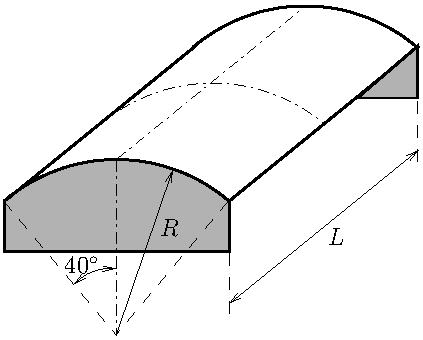
\includegraphics{scordelis}}

Los dos extremos curvos est�n apoyados sobre diafragmas r�gidos que impiden
�nicamente los desplazamientos en direcci�n vertical y permiten los
desplazamientos en horizontal, mientras que
los bordes laterales rectos est�n libres. El conjunto est� sometido a una carga
gravitatoria vertical uniforme, siendo el peso espec�fico del material igual
a $360\,\text{N/m$^3$}$.

Se desea conocer el desplazamiento vertical en el punto medio del borde
libre\footnote{El valor que est� reportado por diversos autores empleando
elementos l�mina es $0.3024$ m. (B�veda de Scordelis-Lo)} y la distribuci�n de
esfuerzos en la cubierta
a lo largo de las lineas de puntos de la figura. Para ello se realizar�n los
siguientes modelos de elementos finitos:
\begin{enumerate}
\item Modelo de elementos s�lidos isoparam�tricos.
\item Modelo de elementos s�lidos de ocho nodos con formulaci�n mixta.
\item Modelo de elementos s�lidos de ocho nodos con formulaci�n de 
deformaciones mejoradas supuestas.
\end{enumerate}
\end{document}
